\documentclass[10pt]{article}

\usepackage{parskip}
\usepackage[margin=1in]{geometry} 
\usepackage{amsmath,amsthm,amssymb, graphicx, multicol, array}
\usepackage[style=apa]{biblatex}
\addbibresource{sources.bib}
\usepackage{enumitem}
\usepackage{tikz}
\usepackage{booktabs}
\usepackage{footmisc}
\usepackage{amssymb}
\usepackage{float}
\usepackage{href-ul}
 
\newcommand{\N}{\mathbb{N}}
\newcommand{\Z}{\mathbb{Z}}
 
\newenvironment{problem}[2][Problem]{\begin{trivlist}
\item[\hskip \labelsep {\bfseries #1}\hskip \labelsep {\bfseries #2.}]}{\end{trivlist}}

\begin{document}
 
\title{Assignment 3 \\Multivariate Time Series Modelling}
\author{Jakob Sverre Alexandersen\\
GRA4159 Trends, Cycles \& Signals Extraction}
\maketitle

The purpose of this assignment is to give you hands-on experience with working with multivariate time series models and prediction as well as common data transformations. We will continue to use the TFP estimates you derived in Assignment 2. 

You have just started in your new job as a macro data scientist in a large international bank with responsibility for tracking the new Norwegian economy. In terms of growth potential, your boss is afraid that Norway is lagging (behind) other countries, and you are asked to start analyzing whether this might be the case. 

\begin{enumerate}
    \item Choose 4 countries that you believe are relevant to compare with Norway and compute
    potential output for each of these countries using the Hamilton filter discussed in class.
    
    Discuss shortly why you chose the countries you did, the data frequency you used, the
    time sample, and the Hamilton filter specification. Plot the potential output estimates for
    all countries in one graph and comment on the result considering your boss' worry.
    \item It is a common assumption that stock market prices contain investors' expectations
    about risk premia and future cash flows. I.e., all else equal, if investors have positive
    expectations about long-run growth potential, stock prices will be high.
    
    Assume that the U.S economy is/has been an engine for global growth. Collect quarterly
    data on the overall stock market valuation for that economy (e.g., \href{https://fred.stlouisfed.org/series/SPASTT01USQ661N}{here}) Also collect (if you have not
    already done so) data and real GDP for mainland Norway at a quarterly frequency.
    \begin{itemize}
        \item Is the data stationary?
        \item Perform ADF tests and comment on the result 
    \end{itemize}
    \item Use the yearly TFP estimate from Assignment 2 and transform it into a quarterly time
    series. Use an interpolation technique of your own choice. Discuss the motivation for
    your choice of method, how you do this, and plot the resulting quarterly series together
    with the stock market index for the U.S. Choose yourself whether you do this in levels or
    growth, or any other transformation, but comment on your transformation and the
    correlation patterns. Are there any signs of co-movement?
    \item Use stationary series for real GDP and TFP in Norway and the stock market in the U.S.
    and estimate a VAR model. Discuss
    \begin{itemize}
        \item The choice of sample and data transformations
        \item The VAR lag length and how you decided on it
        \item Is the VAR stable?
        \item Do you find any sign of Granger-causality?
    \end{itemize}
    \newpage 
    \item Use the same VAR as in (4), but truncate the estimation sample with one year and reestimate the model. Now, produce iterative forecasts for 1-4 quarters and plot the
    forecasts together with the actual realizations for all three variables. Are the predictions
    any good?
\end{enumerate}
\section{Comparing Norway to his less cooler friends}

We're asked to compare Norway with 4 other countries that may be relevant to compare with. There are a couple metrics I want to use to make this battle fair. First, the countries we compare against should have an equal GDP per capita. Secondly, the counterparts should be structurally comparable to Norway (small, open, advanced economies). Some strong candidates here are Sweden and Denmark as our Nordic peers; similar institutions, welfare models and openness. I also choose Switzerland since they're small, open, rich, and a good contrast to Norway's oil dependence (Switzerland is resource-independent). The last peer is the United States of America, as we can use them as the global growth benchmark.

For the analysis I will use growth rates in GDP. GDP growth rates are generally considered stationary, making them an excellent fit for the Hamilton filter. Thus, the filter will separate out the trend component (potential growth rate) from the cyclical component. Note that we are applying the filter to real GDP growth rates rather than log levels, and that the resulting trend estimate represents the evolution of potential growth over time. 

We're using quarterly data, seasonally adjusted from OECD. The common sample is 1961Q1 to 2025Q4, and it spans multiple business cycles, which is good for estimating the Hamilton filter coefficients. In the Hamilton filter, we set $h = 8 $, which corresponds to a 2-year forecast horizon. We set $p = 4 $; 4 lags. Both specifications satisfy Hamilton's recommendation for quarterly data (and that $p > d $). 
\begin{figure}[H]
    \centering
    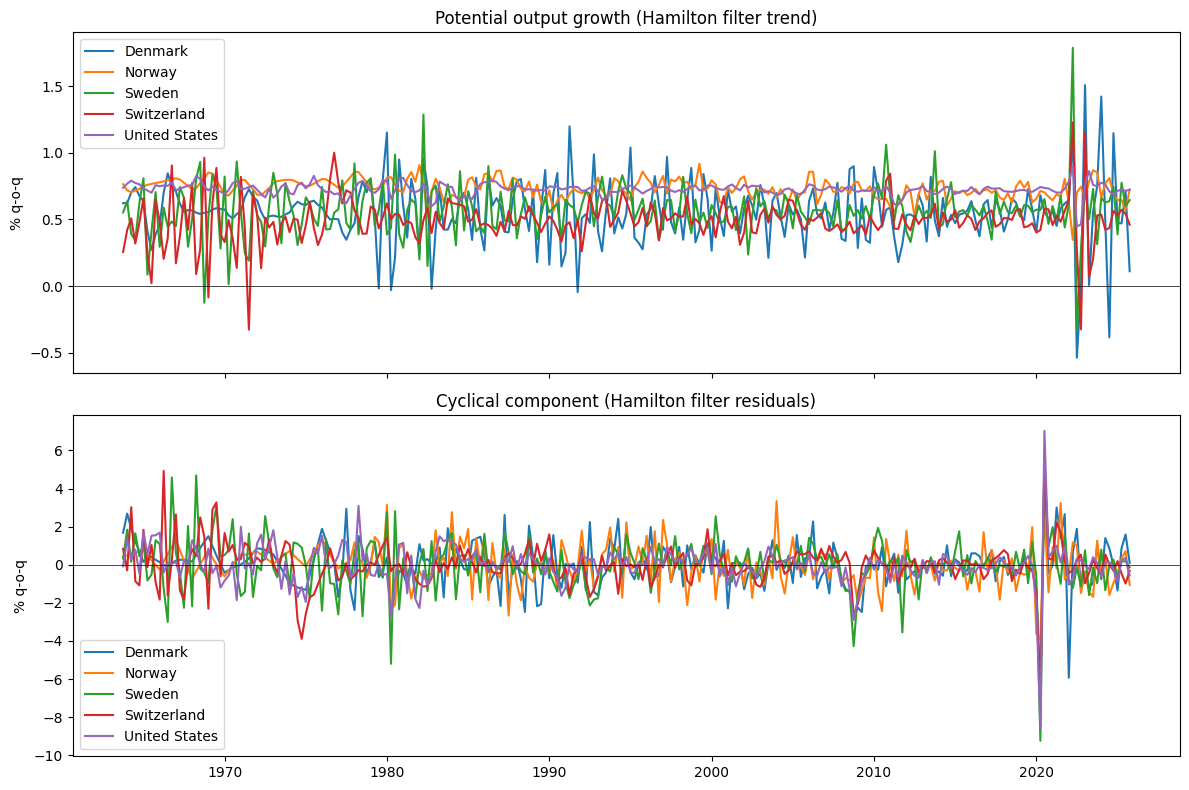
\includegraphics[width=0.9\textwidth]{2026-03-19-09-26-07.png}
\end{figure}
When we look at the full sample, we can see that Norway (orange) actually track remarkably in line with the pack throughout the entire sample. There's no obvious period where Norway is persistently below the others. The US (purple) stands out for being the most stable trend line with very few sharp swings. Switzerland is notably volatile in the early period, with a sharp dip in the early 70s (oil crisis impact on a small open economy). 

If we look at the cycle in the bottom panel, we note that Covid-19 absolutely dominates. Sweden had the largest negative cyclical shock ($\sim - 9\% $), followed by the US and Denmark. Pre-Covid, the usual suspects show up -- recessions at around 1980 and 2008
\begin{figure}[H]
    \centering
    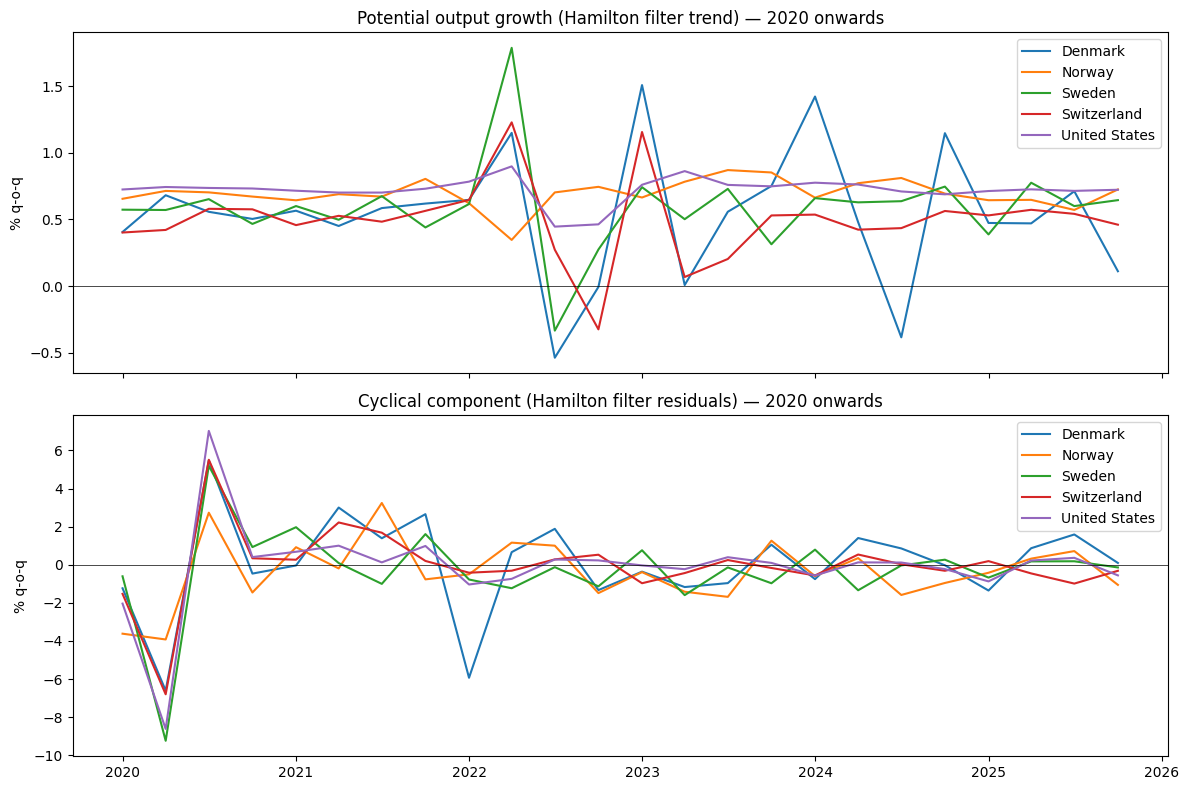
\includegraphics[width=0.9\textwidth]{2026-03-19-09-26-17.png}
\end{figure}
After zooming in to 2020 to date, post-Covid recovery temporarily spiked trend estimates for Sweden ($\sim 1.8\% $ in early 2022), Denmark and Switzerland, but this is an artifact of the filter incorporating the bounce-back. By 2024--2025, all five countries converge back to roughly 0.5--0.7\% q-o-q trend growth. Norway sits comfortably in the middle of the pack, and not visibly below his peers. Denmark is the odd one out, swinging wildly between -0.5\% and +1.5\%, which likely reflects its small economy being sensitive to a few large sectors (shipping and life sciences)

Bottom line, Norway does not seem to be lagging behind its peers. The trend growth estimates show that all five advanced economies have experienced fluctuations around similar levels, with no clear evidence that Norway's potential growth is systematically lower than its peers. The picture is one of convergence across advanced economies rather than Norway specifically falling behind. 
\newpage
\section{On Stationarity}
Looking at the plots, the data is clearly non-stationary in levels. They trend upward with no sign of mean-reversion. 
\begin{figure}[H]
    \centering
    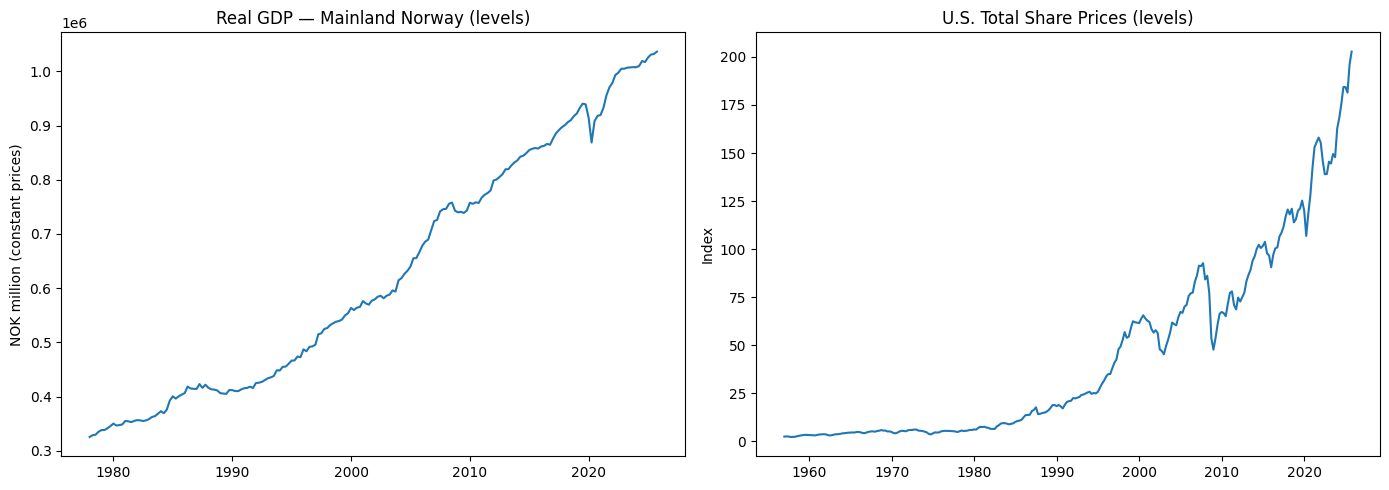
\includegraphics[width=1\textwidth]{2026-03-19-10-28-38.png}
\end{figure}
Now to confirm it with ADF tests. If we look at the levels: 
\begin{center}
    \begin{tabular}{|c|c|c|c|}
        \hline 
        \textbf{Series} & \textbf{ADF Stat} & \textbf{p-value} & \textbf{Verdict}\\\hline 
        Norway GDP levels & 1.53 & 0.998 & Can't reject unit root\\\hline 
        U.S. shares levels & 3.29 & 1 & Can't reject unit root\\\hline 
    \end{tabular}
\end{center}
Both ADF statistics are positive, well above all critical values. The p-values are essentially 1. Clear evidence of unit roots -- both series are non-stationary in levels. 

\textbf{Log levels}
\begin{center}
    \begin{tabular}{|c|c|c|c|}
        \hline 
        \textbf{Series} & \textbf{ADF Stat} & \textbf{p-value} & \textbf{Verdict}\\\hline 
        Norway GDP growth & -14.29 &  0.000 & Reject unit root \\\hline 
        U.S. shares growth & -10.98 &  0.000 & Reject unit root \\\hline 
    \end{tabular}
\end{center}
Massively negative ADF statistics, well below the 1\% critical value. Both reject the null at any conventional significance level. Log-differencing makes both series stationary. 

Both series are $I(1) $ -- integrated of order one. In levels they exhibit clear unit roots (trending, no mean-reversion), but their first differences (log growth rates) are stationary. We must remember this for later tasks, as we must use the stationary growth rate transformations as inputs to the VAR, not the raw levels. 
\newpage 
\section{TFP}
We used cubic spline interpolation to go from annual to quarterly TFP. The reason why we used cubic spline is because TFP is inherently a slow-moving measure of aggregate productivity. It reflects long-run technological change, not quarter-to-quarter fluctuations. Cubic spline preserves this smooth character and avoids artificial jumps at year boundaries that linear interpolation would produce. 

\begin{figure}[H]
    \centering
    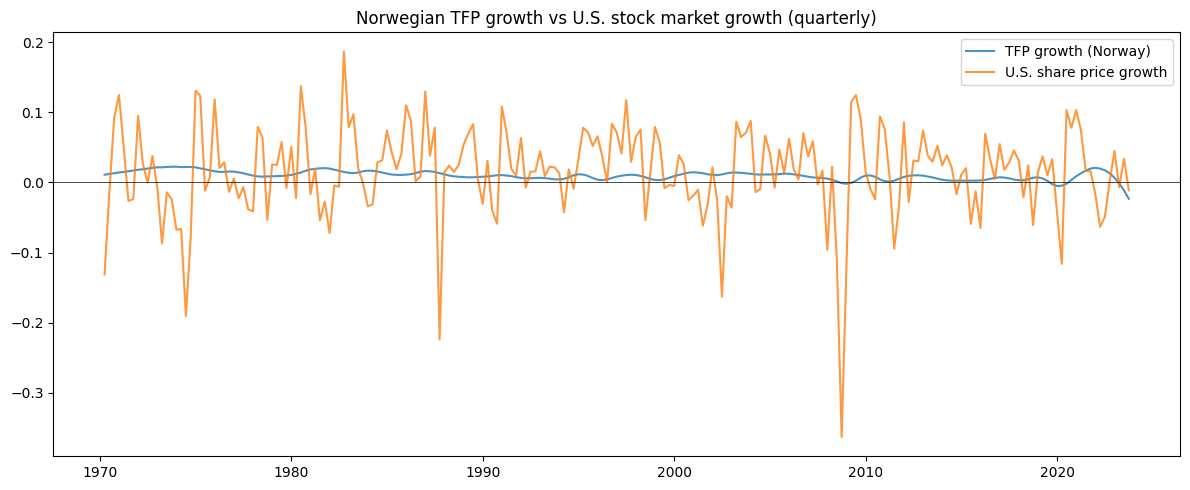
\includegraphics[width=1\textwidth]{2026-03-19-11-35-38.png}
\end{figure}
We plotted log growth rates (first differences of log levels) for both series. This is natural because both series are $I(1) $ in levels (as shown in the previous task). Growth rates are stationary and comparable across series with different units. This transformation is also consistent with what we'll feed into the VAR in the next task. 

The plot shows us that TFP growth (blue) is very smooth and slow-moving, hugging close to zero with tiny fluctuations. This is partly a real feature of TFP (productivity evolves gradually) and partly an artifact of interpolating annual data. The spline can't capture within-year volatility that doesn't exist in the source data. We also see that U.S. stock market growth (orange) is highly volatile with large swings; crashes in the mid-70s, late 1980s, dot-com bust of 2000, 2008 GFE, and 2020 Covid are all clearly visible. There is no visible co-movement between the two series at the quarterly frequency.

The correlation is -0.005, essentially zero. There's no contemporaneous linear relationship between Norwegian TFP growth and U.S. stock price growth at the quarterly frequency. This is not surprising at all, for a couple of reasons. The first is frequency mismatch -- TFP is fundamentally an annual measure that we've interpolated to quarterly. The spline gives us a smooth path, but it can't create genuine quarterly variation. Meanwhile, stock prices fluctuate wildly quarter to quarter. We're comparing a slow-moving signal to a noisy one. 

Secondly, stock prices reflect \textit{expectations} about future cash flows and growth. TFP is computed from \textit{realized} historical data (output, capital, labor). Any relationship between the two would more likely show up with stocks \textit{leading} TFP, not contemporaneously. Lastly, Norwegian TFP reflects the Norwegian production structure; U.S. stocks reflect the American economy. While there may be global linkage, the direct channel is indirect at best. 

The bottom line is that there are no meaningful signs of contemporaneous co-movement, which is consistent with the different natures of these two series (slow-moving backward-looking productivity residual vs. volatile forward-looking asset prices). Any relationship may exist at longer horizons or with lags, which is partly what the next task can explore. 
\newpage 
\section{VAR Model}
We start with the three stationary series -- real GDP growth (mainland Norway), TFP growth Norway, and U.S. stock market growth -- all of whom are in logs. The next step is to select our lag length, we use BIC as our criterion (as it's common in macro), and find that 3 lags is the best. 

We estimate a VAR(3) model using the aforementioned stationary series. The common quarterly sample runs from 1978-04-01 to 2023-10-01, giving 183 observations. With 3 variables and 3 lags, we estimate 10 parameters per equation (9 lag coefficients and 1 constant), leaving ample degrees of freedom. 

We select the lag order using information criteria, evaluating up to 12 lags. BIC selects 3 lags. We proceed with BIC's recommendation, as it penalizes over-parameterization more heavily than AIC and is the standard choice in macroeconomics where parsimony is valued. 

The VAR is stable: all roots of the characteristic polynomial lie outside the unit circle, confirmed by \verb|is_stable()|. This means the system is covariance stationary and shocks to any of the three variables die out over time. The residual autocorrelation plots further support adequate model specification; virtually all autocorrelations fall within the $2/\sqrt{T} $ confidence bands, indicating the residuals are approximately white noise. 
\begin{figure}[H]
    \centering
    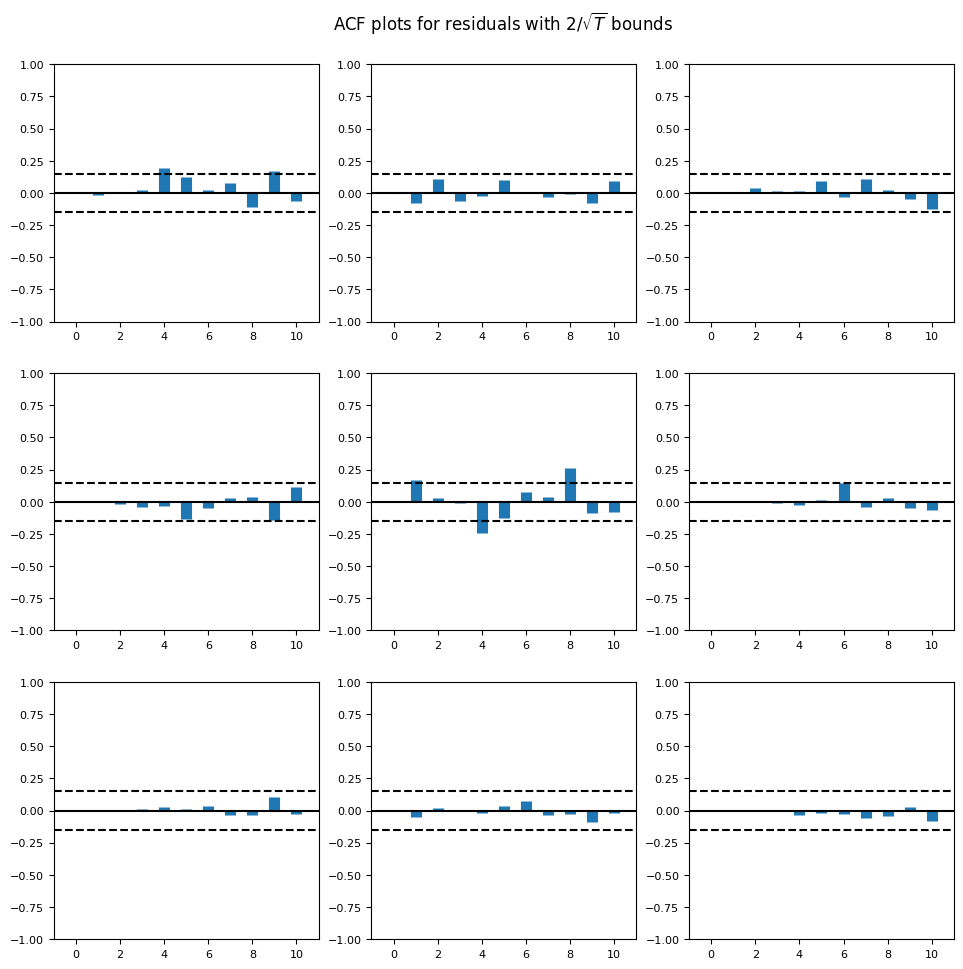
\includegraphics[width=0.9\textwidth]{2026-03-19-13-22-15.png}
\end{figure}
\newpage 
\textbf{Granger causality}
\begin{center}
    \begin{tabular}{|c|c|c|c|}
        \hline 
        \textbf{Direction} & \textbf{F-stat} & \textbf{p-value} & \textbf{Significant? (5\%)}\\\hline 
        TFP $\to $ GDP & 3.11 & 0.026 & Yes \\\hline 
        U.S. stocks $\to $ GDP & 3.62 & 0.013 & Yes \\\hline 
        GDP $\to $ TFP & 0.15 & 0.930 & No \\\hline 
        U.S. stocks $\to $ TFP & 0.14 & 0.935 & No \\\hline 
        GDP $\to $ U.S. stocks & 1.91 & 0.127 & No \\\hline 
        TFP $\to $ U.S. stocks & 0.69 & 0.560 & No \\\hline 
    \end{tabular}
\end{center}
The results reveal an asymmetric predictive structure. Both TFP and U.S. stock returns Granger-cause Norwegian GDP growth; lagged U.S. stock returns in particular carry a positive and significant coefficient at lag 1 ($t = 3.00,\, p = 0.003 $), consistent with the idea that the U.S. stock market contains forward-looking information about global growth that feeds into the Norwegian economy. 

Nothing Granger-causes TFP growth. The TFP equation is almost entirely driven by its own lags (with t-statistics of 46, -22, and 14), which is expected: TFP is interpolated from annual data via cubic spline, making it extremely smooth and autocorrelated. There is simply no room for other variables to add predictive power beyond TFP's own history. 

Similarly, Norwegian variables do not Granger-cause U.S. stock returns. This is economically sensible, as Norway is a small open economy, and its macro aggregate should not drive the world's largest equity market. 

In sum, the VAR supports a narrative where the U.S. acts as a leading indicator for the Norwegian econonomy, but not the reverse. 
\newpage 
\section{VAR Prediction}
We truncate the sample by 4 quarters (one year), re-estimate the VAR(3), and produce iterative forecasts for $h = 1 \text{ to } h = 4 $. The results are mixed. GDP growth forecasts perform well, the forecast errors are small (RMSE = 0.002) and the VAR tracks the actuals closesly across all four horizons. TFP growth forecasts are accurate at $h = 1 $, but diverge as the actual series turns negative while the model, extrapolating the prior upward trend, keeps predicting mildly positive growth. U.S. stock return forecasts are the weakest (RMSE = 0.027), with the VAR converging quickly toward the unconditional mean while actuals swing between +5\% and -1\%; consistent with the well-known difficulty of predicting equity returns. Across all three variables, forecast errors grow with the horizon, and forecasts converge toward their respective means, both of which are standard properties of stationary VAR models. 
\begin{figure}[H]
    \centering
    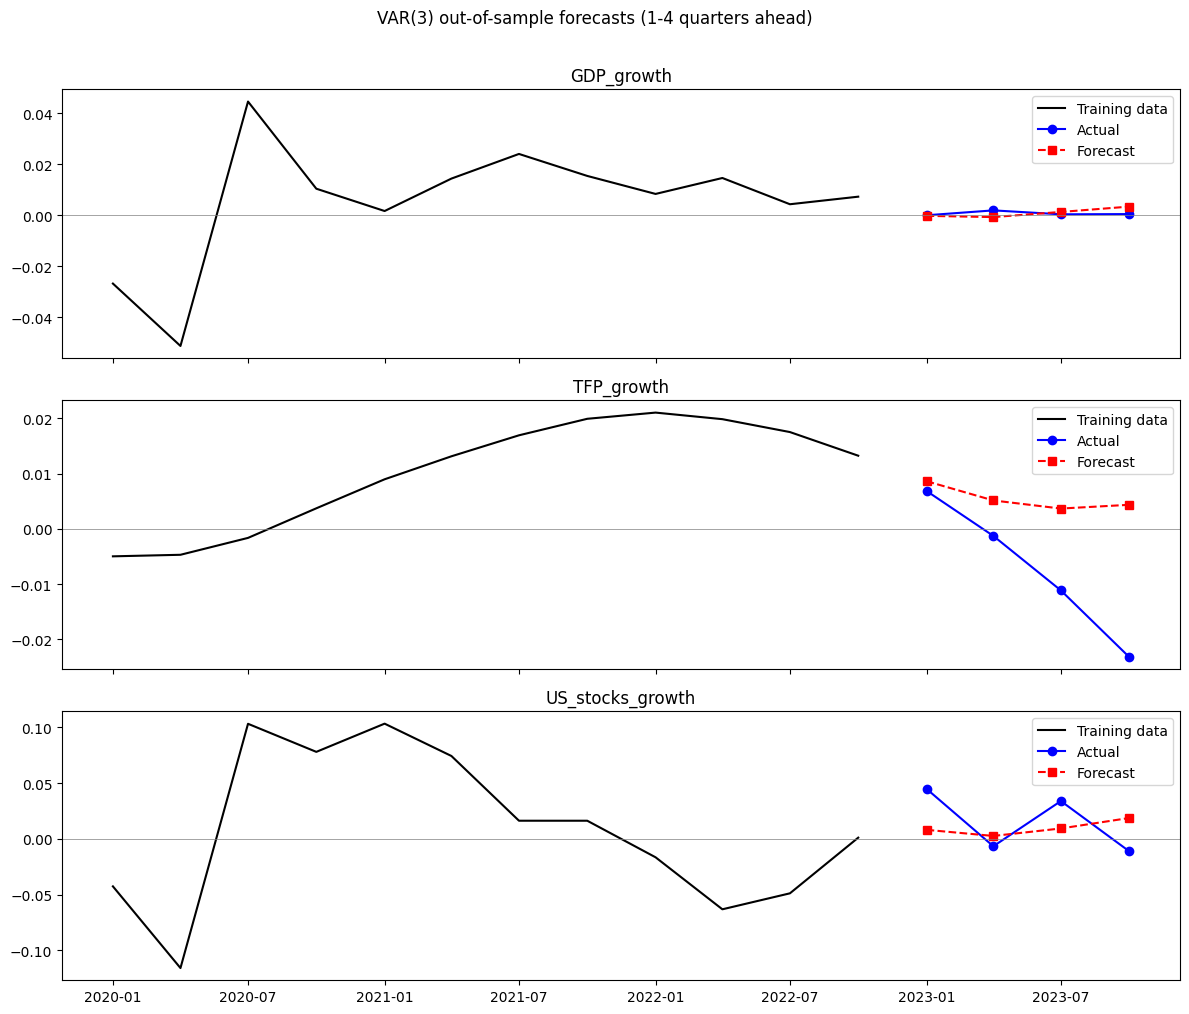
\includegraphics[width=1\textwidth]{2026-03-19-14-29-05.png}
\end{figure}

\newpage 
\printbibliography

\end{document}